\documentclass{article}
\usepackage{tikz}
\usepackage[a4paper]{geometry}
\usepackage{fancyhdr}
\pagestyle{fancy}
\lhead{Gedämpfte Schwingungen}
\rhead{März 2026}
\begin{document}
\section{Gedämpfte Schwingungen}
Eine gedämpfte Schwingungen ist eine Schwingung, welche mit der Zeit gedämpft ist; die Amplitude nimmt mit der Zeit ab.
 
In der Realität ist jede Schwingung, bei welcher nicht konstant Energie von außen hinzugeführt wird, eine gedämpfte Schwingung. Die Amplitude jeder Schwingung sinkt dauerhaft, weil Energie verloren geht. Sei es auch nur die Reibung.
\begin{center}
 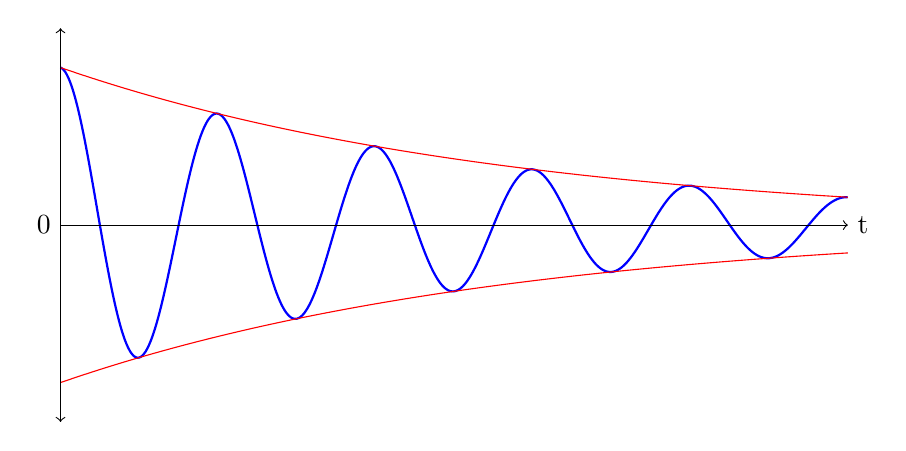
\begin{tikzpicture}     
  \draw[thick, blue, domain=0:10, samples=500]  
            plot (\x, {2^(-0.25*\x) * 2*sin(\x*360 / 2 + 90)});
  \draw[red, domain=0:10, samples=100]  
            plot (\x, {2 * 2^(-0.25*\x)});
  \draw[red, domain=0:10, samples=100]  
            plot (\x, {-2 * 2^(-0.25*\x)});
     
  \draw[->] (0, 0) -- (10, 0) node[right] {t};
  
  \draw (0, 0) node[left] {$0$}; 
  \draw[<->] (0, -2.5) -- (0, 2.5); 
 \end{tikzpicture} 
\end{center} 
\subsection{Mathematisch}  
Die Einhüllende der Maxima und Minima, also auch quasi die Linie, die die theoretische Amplitude an jedem Punkt darstellt, ist eine Funktion des exponentiellen Zerfalls. Die bereits bekannte Schwingungsgleichung wird mit einem Faktor $e^{-kt}$ multipliziert.
 
Dies zeigt auch offensichtlich, dass $T$ konstant bleibt. 
\end{document}